\documentclass{ximera}  


\input{../preamble.tex}



 
\title{Magnetostatics} 
\author{Milica Markovic} 
\outcome{Magnetostatic fields.}
\begin{document}  
\begin{abstract}  

\end{abstract}  
\maketitle    


\section{Static Magnetic Field}

Sources of static magnetic fields are DC currents.

\subsection{What is the source of the magnetic field?}

Magnet. This is the first source of the magnetic field that people have discovered in Greece long time ago. \footnote{to be exact …} Danish scientist Oersted discovered later that the current passing through wire will deflect a compass needle. Later French scientists Biot and Savart quantified this statement:

\begin{eqnarray}
B = \mu_0 \frac{I}{2 \pi r}
\end{eqnarray}

Where B is magnetic flux density, $\mu_0$ is magnetic permeability, I is the electric current, and r is the distance to the point where the magnetic field is measured.

HERE PICTURE WITH A WIRE AND THE magnetic field.



In a magnetic material instead of $\mu_0$ in the above formula we have $\mu=\mu_0 \mu_r$. $\mu_r$ is relative magnetic permeability.

\subsection{Constitutive parameters of a material}

We have introduced two constitutive parameters so far, electric permittivity $\epsilon$ and magnetic permeability $\mu$. The third parameter is conductivity $\sigma$. Conductivity is zero for perfect insulator and infinite for perfect conductor. 

The speed of light in air is equal to 

\begin{eqnarray}
c=\frac{1}{\sqrt{\epsilon_0 \mu_0}}
\end{eqnarray}  

 
\subsection{Charged Particle in a Static Magnetic Field}



\subsection{Force on a conductor carrying current}


\subsection{Wire frame carrying current in a static magnetic field}


\subsection{Biot-Savart's Law}
How to find the magnetic field due to a current distribution.





\subsection{Ampere’s Law}


\subsection{Inductance}
Types, internal external.  Ways to find inductance through energy and directly. What is inductance, how does it affect circuits.

{\large EXAMPLE} Two wire line
{\large EXAMPLE} Coax
{\large EXAMPLE} Internal inductance of wire, block etc.

\subsection{Mutual Inductance}


\begin{figure}[htbp]
\begin{center}
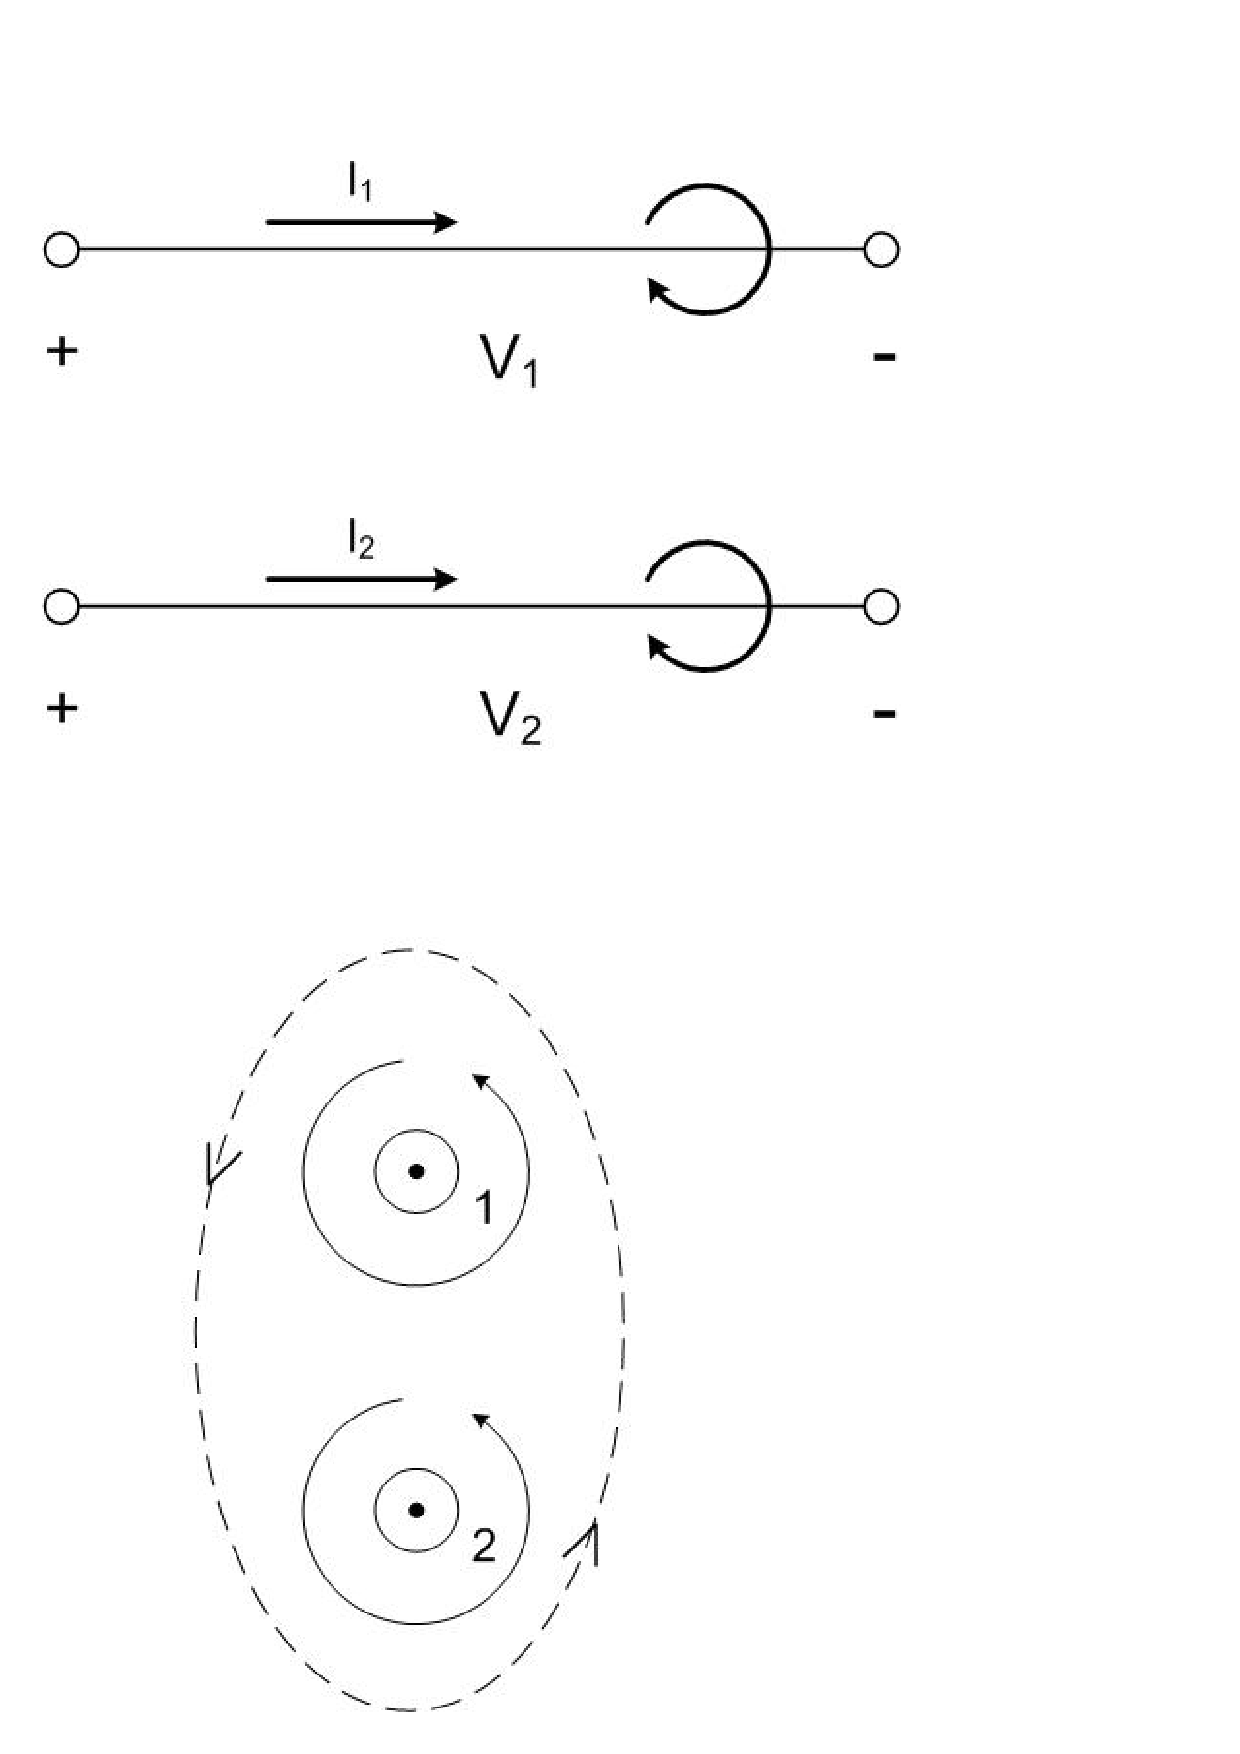
\includegraphics[scale=0.5]{../jpg/increaseinflux.jpg}
\end{center}
\caption{Mutual Inductance: Increasing the magnetic field and therefore current in one wire due to another wire in vicinity. }
\label{MutualInduc}
\end{figure}



\subsection{Inductance in circuit theory}


\begin{figure}[htbp]
\begin{center}
\includegraphics[scale=0.5]{../jpg/CircuitwithInductor.jpg}
\end{center}
\caption{Simple electronic circuit with an inductance and resistance. }
\label{MutualInduc}
\end{figure}










\end{document} 
